\documentclass[a4paper,oneside]{report}

\usepackage{amsmath}
\usepackage{amssymb}
\usepackage{caption}
\usepackage[english]{babel}
\usepackage{fancyhdr} 
\usepackage{float}
\usepackage{multirow}
\usepackage[pdftex]{graphicx}
\usepackage{listings}      
\usepackage{pdfpages}
\usepackage{setspace}
\usepackage{url}
\usepackage{wrapfig}

\lstset{language=Ada,
numberstyle=\footnotesize,
%basicstyle=\ttfamily\footnotesize,
basicstyle=\footnotesize,
numbers=left,
stepnumber=1,
frame= lines,
breaklines=true}

\makeatletter


%
% Some custom definitions
%

% add horizontal lines
\newcommand{\HRule}{\rule{\linewidth}{0.5mm}}
\newcommand{\HRuleLight}{\rule{\linewidth}{0.1mm}}

% custom part page
\def\part#1#2
{
	\par\break
  	\addcontentsline{toc}{part}{#1}
	\noindent
	\null	
	\HRuleLight\\[0.0cm]
	\vspace{20pt}	 
	\begin{flushright} 		
  	{\Huge \bfseries \noindent #1}\\
  	\vspace{30pt} 
	\begin{minipage}{0.85\textwidth}
		\begin{flushright}
		{\large \noindent #2}
		\end{flushright}
	\end{minipage}\\[0.75cm] 
	\end{flushright} 		
	\thispagestyle{empty}
	\break
}

% chapter header
\renewcommand{\@makechapterhead}[1]
{\vspace*{50\p@}{
	\parindent \z@ \raggedright \normalfont
	%\huge \bfseries \thechapter. #1
	\huge \bfseries #1
	\vspace{20pt}}}

\setcounter{secnumdepth}{-1} 
\onehalfspace
\oddsidemargin 1in 
\oddsidemargin 0.6in 
\topmargin -0.3in
\setlength{\textwidth}{14cm}
\setlength{\textheight}{23cm}
\lstset{language=C} 

\begin{document}

%
% Cover page
%
\begin{titlepage}
\begin{center}

\HRuleLight\\[0.5cm]

\Huge Programming, Concurrency and Client-Server Computing

\HRuleLight\\[0.2cm]

\large School of Computing, Engineering and Mathematics\\ \textbf{University of Brighton}

\vfill
\huge Revision Booklet\\
\large May, 2012\\

\end{center}
\end{titlepage}


%
% Table of contents
%
{
	\renewcommand\thepage{}
	\setcounter{tocdepth}{3}
	\tableofcontents
	\clearpage
}

% reset page count
\setcounter{page}{1}


%
% Start of content
%

%\section{What Makes a Good Program}
%\section{History(?)}
\chapter{Programming Languages}

There are many different paradigms in computer programming here are some examples


\begin{description}

\item[Imperative] C
\item[Declarative] SQL, CSS
\item[Object Orientated] Ada, C++, C\#, Java
\item[Logical] Prolog
\item[Functional] Haskell, F\#, Lisp, Clojure (if your a real hipster)

\end{description}


	\section{Typing Systems}

		\subsubsection{Static}

		A programming language is said to use static typing when type checking is performed during compile-time as opposed to run-time. Statically typed languages include ActionScript 3, Ada, C, D, Eiffel, F\#, Fortran, Go, Haskell, haXe, JADE, Java, ML, Objective-C, OCaml, Pascal, and Scala. C++ is statically typed, aside from its run-time type information system. The C\# type system performs static-like compile-time type checking, but also includes full runtime type checking. 

		Static typing is a limited form of program verification (see type safety): accordingly, it allows many type errors to be caught early in the development cycle. Static type checkers evaluate only the type information that can be determined at compile time, but are able to verify that the checked conditions hold for all possible executions of the program, which eliminates the need to repeat type checks every time the program is executed. Program execution may also be made more  efficient (e.g. faster or taking reduced memory) by omitting runtime type checks and enabling other optimisations.


		\subsubsection{Dynamic}
		
		A programming language is said to be dynamically typed when the majority of its type checking is performed at run-time as opposed to at compile-time. In dynamic typing values have types, but variables do not; that is, a variable can refer to a value of any type. Dynamically typed languages include APL, Erlang, Groovy, JavaScript, Lisp, Lua, MATLAB, PHP, Prolog, Python, Ruby, Smalltalk and Tcl.

 	 	Implementations of dynamically-typed languages generally associate run-time objects with "tags" containing their type information. This run-time classification is then used to implement type checks and dispatch overloaded functions, but can also enable pervasive uses of dynamic dispatch, late binding and similar idioms that would be cumbersome at best in a statically-typed language, requiring the use of variant types or similar features.

 		More broadly, as explained below, dynamic typing can improve support for dynamic programming language features, such as generating types and functionality based on run-time data. (Nevertheless, dynamically typed languages need not support any or all such features, and some dynamic programming languages are statically typed.) On the other hand, dynamic typing provides fewer a priori guarantees: a dynamically typed language accepts and attempts to execute some programs that would be ruled as invalid by a static type checker, either due to errors in the program or due to static type checking being too conservative.

 		 Dynamic typing may result in runtime type errors—that is, at runtime, a value may have an unexpected type, and an operation nonsensical for that type is applied. Such errors may occur long after the place where the programming mistake was made—that is, the place where the wrong type of data passed into a place it should not have. This may make the bug difficult to locate.

 		Dynamically typed language systems' run-time checks can potentially be more sophisticated than those of statically typed languages, as they can use dynamic information as well as any information from the source code. On the other hand,  runtime checks only assert that conditions hold in a particular execution of the program, and the checks are repeated for every execution of the program.

		Development in dynamically typed languages is often supported by programming practices such as unit testing. Testing is a key practice in professional software development, and is particularly important in dynamically typed languages. In practice, the testing done to ensure correct program operation can detect a much wider range of errors than static type-checking, but full test coverage over all possible executions of a program (including timing, user inputs, etc.), if even  possible, would be extremely costly and impractical. Static typing helps by providing strong guarantees of a particular subset of commonly-made errors never occurring


		\subsubsection{Strong Vs Weak}
			
		Most generally, ``strong typing" implies that the programming language places severe restrictions on the intermixing that is permitted to occur, preventing the compiling or running of source code which uses data in what is considered to be an invalid way. For instance, an addition operation may not be used with an integer and string values; a procedure which operates upon linked lists may not be used upon numbers. However, the nature and strength of these restrictions is highly variable.

\begin{lstlisting}[label=some-code,caption=Weak Typing] 
a = 2
b = "2"
 
concatenate(a, b) # Returns "22"
add(a, b)         # Returns 4
\end{lstlisting}

\begin{lstlisting}[label=some-code,caption=Strong Typing] 
a = 2
b = "2"
 
concatenate(a, b)     # Type Error
add(a, b)             # Type Error
concatenate(str(a), b) # Returns "22"
add(a, int(b))         # Returns 4
\end{lstlisting}


\section{A comparison between Java, Ada, Haskell and Prolog}


	\subsection{Java}
	
	Java is a static, Object Orientated , structured, imperative, generic, reflective generic reflective language. 
	
	The language derives much of its syntax from C and C++ but has a simpler object model and fewer low-level facilities. Java applications are typically compiled to bytecode (class file) that can run on any Java Virtual Machine (JVM) regardless of computer architecture. Java is a general-purpose, concurrent, class-based, object-oriented language that is specifically designed to have as few implementation dependencies as possible. It is intended to let application developers "write once, run anywhere" (WORA), meaning that code that runs on one platform does not need to be recompiled to run on another. Java is currently one of the most popular programming languages in use.
	
	
	\begin{itemize}
	\item Multi threading
	\item Networking Libraries
	\item Platform Independent GUI (SWING)
	\item Large standardized class library
	\end{itemize}
	

	\subsection{Ada}

	Ada is a Multi-paradigm structured, statically typed, imperative, wide-spectrum, and object-oriented high-level computer programming language, extended from Pascal and other languages. It has strong built-in language support for explicit concurrency, offering tasks, synchronous message passing (via guarded task entries), protected objects (a monitor-like construct with additional guards as in conditional critical regions), and nondeterminism (via select statements).

	Ada was originally designed by a team led by Jean Ichbiah of CII Honeywell Bull under contract to the United States Department of Defense (DoD) from 1977 to 1983 to supersede the hundreds of programming languages then used by the DoD. Ada is strongly typed and compilers are validated for reliability in mission-critical applications, such as avionics software.


Ada's type system is not based on a set of predefined primitive types but allows users to declare their own types. This declaration in turn is not based on the internal representation of the type but on describing the goal which should be achieved. This allows the compiler to determine a suitable memory size for the type, and to check for violations of the type definition at compile time and run time (i.e. range violations, buffer overruns, type consistency, etc.). Ada supports numerical types defined by a range, modulo types, aggregate types (records and arrays), and enumeration types. Access types define a reference to an instance of a specified type; untyped pointers are not permitted. Special types provided by the language are task types and protected types.


	\begin{lstlisting}[label=Date Type,caption=Ada Date Type] 

type Day_type   is range    1 ..   31;
type Month_type is range    1 ..   12;
type Year_type  is range 1800 .. 2100;
type Hours is mod 24;
type Weekday is (Monday, Tuesday, Wednesday, Thursday, Friday, Saturday, Sunday); 
 
type Date is
   record
     Day   : Day_type;
     Month : Month_type;
     Year  : Year_type;
   end record;


	\end{lstlisting}



	Ada programs consist of packages, procedures and functions.

	Packages, procedures and functions can nest to any depth and each can also be the logical outermost block.

	Each package, procedure or function can have its own declarations of constants, types, variables, and other procedures, functions and packages, which can be declared in any order.

	\begin{lstlisting}[label=Ada Package Specification,caption=Ada Package Specification] 
package Example is
     type Number is range 1 .. 11;
     procedure Print_and_Increment (j: in out Number);
end Example;
	\end{lstlisting}


\begin{lstlisting}[label=Ada Package Implementation,caption=Ada Package Implementation] 
with Ada.Text_IO; 
package body Example is

i : Number := Number'First;

procedure Print_and_Increment (j: in out Number) is

function Next (k: in Number) return Number is
begin
return k + 1;
end Next;

begin
Ada.Text_IO.Put_Line ('The total is: ' & Number'Image(j));
j := Next (j);
end Print_and_Increment;

begin
while i < Number'Last loop
Print_and_Increment (i);
end loop;
end Example;
\end{lstlisting}

	\subsection{C++}

	C++ is a statically typed, free-form, multi-paradigm, compiled, general-purpose, powerful programming language. It is regarded as an intermediate-level language, as it comprises a combination of both high-level and low-level language features. It was developed by Bjarne Stroustrup starting in 1979 at Bell Labs object oriented features such as classes to the C programming language. Originally named C with Classes, the language was renamed C++ in 1983, as a pun involving the increment operator.

 	C++ is one of the most popular programming languages implemented on a wide variety of hardware and operating system platforms. As an efficient compiler to native code, its application domains including systems software, application software, device drivers, embedded software, high-performance server and client applications, and entertainment software such as video games. Several groups provide both free and proprietary C++ compiler software, including the GNU Project, Microsoft, Intel and Embarcadero Technologies. Java and C\# which have become popular alternatives evolved from C++, but make extensive use of automatic garbage collection and compiling to an intermediate machine-independent intermediate code.
	

	\begin{itemize}
	\item Operator Overloading
	\item Templates/ Generic programming
	\item Encapsulation (Hiding information dependent on scope, private, public etc.)
	\item Inheritance
	\item Standardized class libraries (Stabdard Template Libary (STL), Core Library)
	\item Pointer arithmetic and manipulation 
	\item Multithreading possible however this often requires an external library such as OpenMP or Boost C++
	\end{itemize}



	\subsection{Haskell}


	Haskell is a functional, lazy/non-strict, modular language.

	Haskell features lazy evaluation, pattern matching, list comprehension, type classes, and type polymorphism. It is a purely functional language, which means that in general, functions in Haskell do not have side effects. There is a distinct type for representing side effects, orthogonal to the type of functions. A pure function may return a side effect which is subsequently executed, modeling the impure functions of other languages.

	Haskell has a strong, static type system based on Hindley–Milner type inference. Haskell's principal innovation in this area is to add type classes, which were originally conceived as a principled way to add overloading to the language, but have since found many more uses.

	The type which represents side effects is an example of a monad. Monads are a general framework which can model different kinds of computation, including error handling, non-determinism, parsing, and software transactional memory. Monads are defined as ordinary datatypes, but Haskell provides some syntactic sugar for their use.
	

	\begin{itemize}
	\item Recursion over iteration, Haskell does not have loops and because of this it uses recursion iterate through lists. Haskell makes use of tail cull recursion which allows the program to recurse indefinitely with out causing a stack overflow that would occur in traditional imperial and object orientated languages.
	
	\item Sparks, Haskell Threads and Worker threads. Haskell deals with concurrency in a unique way. when a task is to be performed it turned into a spark. A Spark is a essentially a task that is added to a task queue.  There sparks are then ignited by Haskell's threads which are then actioned by a worked thread. This way of delegating tasks offerers very efficient multi core performance which very minimal over head in code due to the fact the complex delegation of how to perform tasks is calculated automatically.

	\end{itemize}
	


	\subsection{Prolog}
	Prolog is a dynamically typed,general purpose logic programming language associated with artificial intelligence and computational linguistics. In Prolog logic is expressed as sets of facts and rules.
	
	Prolog features a built in back tracking engine which allows of easy evaluation of large rule sets, this gives Prolog a form of overloading on rules. 
	
	Prolog is tail call recursive with iteration handled in a similar way to Haskell.
	
	Prolog has many different implementations SWI-Prolog and Win-Prolog are two of these. Some Prolog implementations support networking which allow the creation of distributed systems. 


\chapter{Concurrency}
	\section{What it is}
	
	Concurrency allows you to effectively utilise available processing power by allowing a computer to perform several different tasks simultaneously (e.g web web server requests, spell-checking whilst typing)
	
    	\subsection{Types of concurrency}
    	
    	\paragraph{Coroutines} With co-operative schedules (or coroutines), processes suspend voluntarily  when they need to wait for an event. Processes may also suspend at regular intervals during lengthy processing.
    	
    	\paragraph{Timeslicing} With pre-emptive scheduling (or timeslicing), processes are suspended as a result of interrupts from external hardware. This can present problems with shared resource access, as it is impossible to predict at what point a process will be suspended.
    	
  	\section{How it's implemented}
  	
    	\subsection{Java}
      		
      		\paragraph{Threads} Java's \emph{Thread} class can be used to implement concurrency. Each instance of the class represents a different `thread' of execution, allowing multiple processes to execute simultaneously.\\ 
\textbf{Useful methods:} \emph{Thread.start()}, \emph{Thread.run()} - thread halts on exit from run, \emph{Thread.sleep(time)}, \emph{Thread.interrupt()}, \emph{Thread.get/setPriority()}

      		\paragraph{Synchronisation} Problems will occur if two threads try to modify/access shared data simultaneously (or rather if one tries to access while one tries to modify, or both try to modify). Using a \emph{synchronized} block prevents data corruption, as only one thread is able to execute it at a time. Each Java object has an internal ‘lock’ and a queue for waiting threads; if the lock is clear, lock the object and enter the block, if the lock is set, wait. On exit from the block, clear the lock and wake up a waiting thread (if there are any). This isn't very OO, as data is only protected where it is accessed, not where it is defined. The solution is to `synchronize' an entire method.
      		
    	\subsection{Ada}
    	
      		\subsubsection{Tasks}
      		Tasks are Ada's equivalent of Java's threads; each separate task representing a separate `thread' of execution. Tasks can communicate with each other via `entry' calls. Entry points are declared in the task spec
– a task declares ‘entries’ (like procedures) in the task spec in the form of ‘accept’ statements. An entry call causes a ‘rendezvous’ between the called task and its caller. The caller waits for the task to accept the call – the accept statement waits for a call (see Listing).
         
\begin{lstlisting}[label=some-code,caption=Ada's Accept Statement] 
loop 
	select
		accept Show (Message : in String) do
			Put_Line(Message);
		end Show; or
		accept Stop;
        exit;
	end select;
end loop;
\end{lstlisting}
      		
      		Entries require a client/server relationship, as they only communicate between one task and another. This is inefficient when just accessing shared data (tasks must be rescheduled to actually pass the data).
      		
      		\subsubsection{Protected records}
      		Protected records (added in Ada 95) use shared data much more efficiently. Protected records contain private data which is accessed by public functions, entries and procedures.\\
      		
      		\noindent\textbf{Functions} are given read-only access to the data and can be executed by multiple tasks simultaneously.\\
      		
      		\noindent\textbf{Procedures} have read and write access to the data, but can only be executed by a single task at any one time. Additionally, no other tasks can be executing any other functions, procedures or entries while a procedure is executing.\\
      		
      		\noindent\textbf{Entries} are similar to procedures, but also has a guard condition which suspends the caller until it evaluates to true. 
      		
    	\subsection{Haskell}

		Haskell supports both pure parallelism and explicit concurrency, however as rule of thumb use Pure Parallelism if possible, otherwise use Concurrency.

		\subsubsection{Parallelism}

			Pure parallelism (Control.Parallel), can be used to speed up pure (non-IO) parts of the program by speeding up a pure computation using multiple processors. Pure parallelism has these advantages:
				\begin{itemize}
					\item Guaranteed deterministic (same result every time)
					\item no race conditions or deadlocks
					\item Software Transactional Memory (STM)
				\end{itemize}


The following code has been parallelized in haskell, this has been done do by importing the Control.Parallel libary and by using \textbf{par} and \textbf{pseq} combinators. 

\textbf{par} tells the compiler that the values can be calculated in parallel

\textbf{pseq} forces the evaluation of c 


\begin{lstlisting}[label=some-code,caption=Parallel code in haskell] 


import Control . Parallel

main = a `par ` b `par ` c `pseq ` print (a + b + c)
where a = ack 3 10
b = fac 42
c = fib 34

fac 0 = 1
fac n = n * fac (n -1)

ack 0 n = n +1
ack m 0 = ack (m -1) 1
ack m n = ack (m -1) ( ack m (n -1) )

fib 0 = 0
fib 1 = 1
fib n = fib (n -1) + fib (n -2)



\end{lstlisting}



			\textbf{Map} is a high order function that applied a given function to each element in a list, this is often referred to as \emph{apply-to-all} , In haskell this is written as map \emph{function} list.



			\textbf{Reduce} also known as fold, is a method of optimizing operations on lists for instance. 

			The folding of the list [1,2,3,4,5] with the addition operator would result in 15, the sum of the elements of the list [1,2,3,4,5]. To a rough approximation, one can think of this fold as replacing the commas in the list with the + operation, giving 1 + 2 + 3 + 4 + 5.

			In the example above, + is an associative operation, so the final result will be the same regardless of parenthesization, although the specific way in which it is calculated will be different. In the general case of non-associative binary functions, the order in which the elements are combined may influence the final result's value. On lists, there are two obvious ways to carry this out: either by combining the first element with the result of recursively combining the rest (called a right fold), or by combining the result of recursively combining all elements but the last one, with the last element (called a left fold). This corresponds to a binary operator being either right-associative or left-associative, in Haskell's or Prolog's terminology. With a right fold, the sum would be parenthesized as 1 + (2 + (3 + (4 + 5))), whereas with a left fold it would be parenthesized as (((1 + 2) + 3) + 4) + 5.

			 In practice, it is convenient and natural to have an initial value which in the case of a right fold is used when one reaches the end of the list, and in the case of a left fold is what is initially combined with the first element of the list. In the example above, the value 0 (the additive identity) would be chosen as an initial value, giving 1 + (2 + (3 + (4 + (5 + 0)))) for the right fold, and ((((0 + 1) + 2) + 3) + 4) + 5 for the left fold.
			


      		\subsubsection{Concurrency}
			Concurrency (Control.Concurrent): Multiple threads of control that execute "at the same time".

				\begin{itemize}
					\item Threads are in the IO monad
					\item IO operations from multiple threads are interleaved non-deterministically
					\item communication between threads must be explicitly programmed
					\item Threads may execute on multiple processors simultaneously
					\item Dangers: race conditions and deadlocks
				\end{itemize}

    	
  	\section{Issues Associated With Concurrency}
  	
  	Although concurrency adds the power to do new things, it also brings with it new types of errors.
  	
    	\subsection{Deadlock}
    	Deadlock occurs when two (or more) processes require access to an inaccessible certain resource in order to continue. This usually occurs when one process has a lock on some resource which is needed by another process, which itself has a lock on a resource which the first process holds. Neither process are   able to relinquish their lock on the problem resources, as they cannot get a lock on the new resources etc. etc.\\
    	
    	\noindent All four of the following conditions are necessary for deadlock to occur: 
    	\begin{enumerate}
    		\item Tasks need to use a non-shareable resource\\ 
    			  \emph{Can be prevented by virtualising resources (e.g. print spooling on disk: printer is non-shareable, disk is shareable), though this is not always possible (e.g. a railway track is not shareable between two trains and cannot be virtualised).}
    		\item Tasks hold onto resources while waiting for extra ones\\
    			  \emph{Insist that all resources are allocated at once (task cannot proceed until all resources have been granted). This is inefficient as resources will be allocated when not needed.}
    		\item Resources cannot be taken away from tasks by a third party\\
    			  \emph{See above solution.}
    		\item There is a circular chain of tasks requesting a resource held by another task\\
    			  \emph{Resources can be prioritised, allocated in priority order. A process must finish using (and release) high priority resources before it can use a lower priority one.}
    	\end{enumerate}
    	
    	It is not always possible to recover from deadlock. The operating system may check for deadlocks by checking the thread table for circularities. If a deadlock is detected, the OS will kill one of the locked processes until the deadlock is broken. This can obviously have severe implications for the program. Similarly, if deadlocks are not dealt with within the program, it may become unresponsive, forcing the user to kill the program manually.
    	
    	\subsection{Livelock}
    	Livelock is similar to deadlock, except that tasks are still able to proceed. However, execution is useless in that tasks will not be able to make any meaningful progress. For example, ethernet, where collisions cause back-offs of exponentially increasing length (this variation in wait time will normally eventually break the lock). Where contention is low, probability of livelock is low enough to ignore (although this is not a suitable response in safety-critical situations). Livelock isn't as easily definable as deadlock, the system may appear to be functioning. Deadlocked threads cannot be scheduled, whereas livelocked ones can. If a `fair' scheduling algorithm is used, livelock can be avoided (e.g. if a guarantee is made that every request is eventually dealt with). 
    	
    	\subsection{Starvation}
    	Starvation occurs if one or more tasks are `starved' of resources by other tasks. This might result from a poor choice of task priorities so that high priority tasks will hog resources that lower priority tasks also need, meaning that the lower priority tasks are never able to function. Even if the high-priority thread is blocked, the low-priority thread still can’t get hold of the resource it needs.
    	
    	\subsection{Priority inversion}
    	This occurs if a high-priority task (A) is unable to access a resource which is held by a lower-priority task (B). If A suspends until the resource is free, B is able to proceed. This means that a low-priority process is taking precedence over a high-priority process. If thread A waits in a loop for the resource, the result is a perpetual livelock: B never runs because A is running, but A is always waiting for B.
    	
    	\subsection{The Dining Philosophers}
    	\begin{quotation}\emph{
    	Five philosophers go to a Chinese restaurant and are seated round a circular table.  There is a single chopstick between each pair of philosophers. Each philosopher alternately thinks (which involves putting down any chopsticks that the philosopher is holding) and eats (which involves picking up two chopsticks - only one chopstick can be picked up at a time).}
    	\end{quotation}
    	
    	The dining philosophers is an example of a problem which exhibits the main dangers associated with concurrent systems. \textbf{Deadlock:} Each philosopher picks up left chopstick and waits forever for the right chopstick to reappear. \textbf{Livelock:} Same as above, but put down left chopstick if right one is unavailable. \textbf{Starvation:} Two philosophers can starve another sitting between them if they are never thinking at the same time\\
    	
\textbf{Solving the problem:} Deadlock can be avoided by providing one extra chopstick or one fewer chair, having one left-handed philosopher, allowing philosophers to snatch chopsticks from each other, philosophers put chopstick down if the other isn’t available, or allowing chopsticks to be shared.   
    	 
 	 	Livelock only requires circular waiting for unshareable resources, so can be avoided by picking up left chopstick and put it down again if chopstick not available, or snatching chopstick from neighbours.
    	 
Another solution could be to provide a bottle of soy sauce, whereby philosophers can only pick up chopsticks if they have the bottle, sauce is put down sauce after both chopsticks are collected. The bottle ensures mutual exclusion for the critical act of picking up a chopstick.
    	
\chapter{Distributed Systems}

	\section{Multi-processors}
	
	Are becoming increasingly common due to their decreasing cost; adding extra processors (or cores) is a much more cost-effective way of increasing performance. Many embedded real-time systems are ad-hoc distributed systems, configuration determined by overall structure of system being controlled (e.g. aircraft: cockpit systems, fuel systems, wings, tailplane). Processors must be located where they are needed and networked together.
	
    	\paragraph{Tightly coupled}	Multiple processors sharing a single memory (e.g. SMP, quad Pentium motherboards). Tightly coupled systems are good for performance (i.e. more processors = faster), but bad for fault tolerance, as the system relies on shared resources. Tightly coupled systems require simpler coordination of tasks, as have shared memory (using some form of semaphore system).
    	
    	\paragraph{Loosely coupled} Distributed networks with no shared memory, with nodes (processors) communicating over a Local Area Network. This makes coordination more difficult (as there's no shared memory), but also means that fault tolerance is possible by introducing duplicate nodes. An issue which is introduced with loosely-coupled systems is that of whether to use homogenous (with identical processors) or heterogenous (different processors) systems. Homogenous processors are able to compare results at regular intervals, using a `majority' voting process allows any failing nodes to be identified. However, if the voting is done through a central unit, failures in that unit will fail the whole system. This can be solved using a distributed analog voting mechanism whereby each unit generates an analog signal (e.g. a voltage) which is applied to one or more common carriers. The resultant voltage indicates result. Introducing heterogenous systems can introduce extra communication difficulties based on the systems' architecture (e.g. using big endian vs. little endian). Fault tolerance is also more difficult, as processor speeds will likely vary, development costs are much higher, and truly independent development is difficult to achieve.
    	
    	\paragraph{Example Use-case: The (Now Defunct) Space Shuttle} 
    	Uses four main processors in a homogenous system, and uses majority voting. If one processor fails, it leaves three others while it is being replaced, the remaining three can continue majority voting. Also has one heterogenous backup processor which is used in emergencies when two of the four main processors have failed (kept as a warm standby, monitoring the main processors to keep up to date).
    	
   	\subsection{Problems}
   	
   	Distributed systems introduce a number of issues which must be addressed in order to work successfully.  One of these issues is global state; for a distributed system to work effectively, there must be shared memory or global state. There also needs to be some common timebase so that the order in which events occur can be determined. Among other things, this is required in order to `snapshot' the complete system in its current state.
   	
	Another big problem with distributed systems is that they are nondeterministic (i.e. the outcome can be unpredictable due to timing issues). There are two types of nondeterminism: angelic (an ‘angel’/external agent ensures that the best choice is always made), and demonic (no assumption can be made about the choice the ‘demon’ will make). Angelic determinism is generally impossible to achieve, were it possible, any NP-complete problem could be solved in polynomial time by always selecting the ‘correct’ path to follow. The alternative is to add mechanisms to make things deterministic.   
   	
   		\paragraph{Issues to be addressed:}
		\begin{itemize}
			\item Ensuring a consistent timebase so that all processors can tell what order events occur in.
			\item Ensuring shared resources are not accessed by multiple processors at the same time (distributed mutual exclusion).
			\item Need to be able to recognise situations where one processor deadlocks another (distributed deadlock detection).
		\end{itemize}
   	
   	\textbf{Failure modes}: transient, permanent, intermittent; fail safe (known state), fail soft (‘graceful degradation’); fail uncontrolled, fail late (correct values but too late), fail silent (no values), fail stop (no values, failure visible to other nodes)
   	\emph{Uncontrolled intermittent failures are the hardest to deal with, as parts of the system will act `traitorously'}

		\subsection{Global Time}
   	
   		Due to unavoidable communication delays, it is impossible to determine absolute time on any node. In most cases, it is sufficient to simply have a correct list of the order in which events occur within the system (generally absolute time doesn't matter). This sequence can be used to number events and provide a non-absolute timestamp. As an example, determining if event A happened before event if A and B originate from the same node and timestamp A < timestamp B then yes, also yes if A is a message being sent and B is that message being received, yes if timestamp A < timestamp C and timestamp C < timestamp B. Otherwise, we don’t know. Upon receipt of a message, the local timestamp is incremented to be higher than that of the incoming message (this technique only suitable for two nodes). 
   
   	With networks of more than two nodes, `vector clocks' can be used. With vector clocks, each node maintains a vector of timestamps, one for each node. Along with each message, a complete vector is also sent. The receiver of the message updates their own vector so that each timestamp is greater than the one in the message
      	
    	\subsection{Network issues}
    	With regards to network issues, we must assume that the communications network is reliable (i.e. any messages sent will eventually be received). This can be done by requiring acknowledgements of all messages (if no acknowledgement of a message is received, the message is sent again). If errors occur (e.g. the message may get lost so the message is sent again, or the reply may get lost so a duplicate message is received). To deal with this, messages are given a unique `sequence' number to uniquely identify it. This can be used to discard any duplicate messages and keep messages in sequence.
    	
    	\subsection{Mutual exclusion}
    	Mutual exclusion is needed to ensure that shared resources are not accessed by multiple nodes simultaneously. Each node is required to keep a queue of pending requests, with the resource being locked in timestamp order. Every request needs to be sent to every other node so that every node’s queue is the same. A node will be able to lock a resource if it's request is first in the queue, and a message has been received from all other nodes with a timestamp greater than the request. This second condition guarantees that no earlier request will still be on its way.
    	
    	\subsection{Deadlock}
    	There may be an inconsistent view of the system due to a lack of global time. For example, node A may report it has resource X and is waiting for Y, while node B may report it has resource Y and is waiting for X (these may not relate to the state of the system at the same time). This could be solved using a centralised algorithm (deadlock detector), with messages to the detector consisting of two parts: a table of threads waiting for node’s resources, and a table of resources waited for by node’s threads. These messages can be compared to check consistency. Each message essentially acting as a snapshot of the current system's threads/resources a a particular moment (like version control). Another approach could be to use a decentralised algorithm to create a trade dependancy chain: thread A requests X, but X is held by B. B is waiting for Y, but Y is held by C, C is waiting for etc. etc. 
    	
    	\subsection{Fault Tolerance}
    	Even with these measures in place, faults can (and do) occur in these circumstances, it's importance to have some error detection/recovery in place. Communication between nodes can fail (i.e no more messages are received, or messages can be garbled). A checksum can be used in these circumstances to verify that the received message is in fact the same as that sent. The nodes themselves can also fail (generating faulty/incorrect messages), to detect this, each node can be compared agains the others.
	
  	\subsection{Distributed Processing}
  	Distributed processing allows processing to be carried out on a remote server. Two varieties considered here:
  	
	  	\subsubsection{Remote Procedure Calls}
		RPC is an inter-process communication that allows a computer program to cause a subroutine or procedure to execute in another address space (commonly on another computer on a shared network) without the programmer explicitly coding the details for this remote interaction. That is, the programmer writes essentially the same code whether the subroutine is local to the executing program, or remote.\\
		
		\noindent \textbf{The RPC Procedure:}
		\begin{enumerate}
			\item The client calls the client stub. The call is a local procedure call, with parameters pushed on to the stack in the normal way.
			\item The client stub packs the parameters into a message and makes a system call to send the message. Packing the parameters is called marshalling.
			\item The client's local operating system sends the message from the client machine to the server machine.
			\item The local operating system on the server machine passes the incoming packets to the server stub.
			\item The server stub calls the server procedure. The reply traces the same steps in the reverse direction (server `unmarshalls' parameters and calls the corresponding procedure).
			\item The server returns the results in a message to the client.
		\end{enumerate}
		
		\noindent \textbf{Data Representation Issues Associated With RPC:}
		\begin{itemize}
			\item Different formats on different machines
			\item Pointers lose their meaning if sent to a remote machine
		\end{itemize}
		
		\emph{To overcome this, the platform-independent External Data Representation (XDR)can be used for common data types. Another solution is to linearise linked data structures.}
  	
  		\subsubsection{Remote Method Invocation}
  		RMI is a Java-specific implementation of RPC. There aren't any issues with data representation: any `serializable' Java objects can be sent. Although Java uses references (pointers) to refer to objects, serialization linearises embedded references automatically. The client accesses `registry server' to get a remote object that implements a desired interface. The client can call methods of this object as it it were a local object.\\
  		
  		\noindent To implement, simple extend \emph{Remote}, and add \emph{RemoteException} handling.
  		
\begin{lstlisting}[label=some-code,caption=Implementing RMI] 
/**
 * The interface
 */
import java.rmi.*;
import java.rmi.server.*;
   
public class Adder extends UnicastRemoteObject implements Adding 
{
    public Adder () throws RemoteException { }
    		
  	public int add (int a, int b) throws RemoteException
	{ return a + b; }
}
  			
/**
 * The server class
 */
import java.rmi.*; 
  		
public class AddServer 
{
	public static void main (String args[]) throws Exception 
	{
		Naming.rebind ("Adder", new Adder()); 
	}
}

/**
 * The client class
 */	
import java.rmi.*;

public class AddClient 
{
    public static void main (String args[]) throws Exception 
	{
      	Adding adder = (Adding)Naming.lookup("//192.168.11.3/Adder");
		System.out.println(adder.add(123,456));
	}
}
\end{lstlisting}
  	
    	\subsection{Distributed Object Frameworks}
    	There are a number of higher-level mechanisms for distributing objects in an object-oriented system. Below are some examples.
    	
      		\subsubsection{Common Object Request Broker Architecture}
      		 Defined by a consortium including IBM, Apple and Sun, CORBA is designed for use on heterogenous systems. It's similar to RPC, may be different hardware, different languages. CORBA uses an Interface Definition Language (IDL) to define objects in a platform-independent way. ORB (Object Request Broker) is used to handle communication with remote objects (lookup service returns references to remote objects, a client-side stub/`proxy' marshals parameters etc. Interface repository allows objects to be located by the interfaces they implement
      		
      		\subsubsection{Jini}
      		A Java-specific framework that uses RMI to build ‘federations of services’. A lookup service locates objects implementing a particular interface. It returns a ‘proxy object’ to communicate with the real object, the proxy can perform a mixture of client-side and server-side processing. Access to Jini services is based on leases (a lease entitles you to use the service for a particular period of time). You can be given exclusive access to the service, or non-exclusive access to allow the same resource to be shared concurrently with others.
      	 
      	 	\paragraph{Proxies}
      	 	Jini uses two styles of proxy: a thin proxy, where everything is passed to the remote object, and a fat proxy where some local processing is performed before passing the request to the remote object. The proxy can validate parameter values before passing them to the remote object, which means more responsiveness at the client end (no waiting for a remote server to tell you that a value is out of range). It also means less loading at the service end (no need to validate parameters sent by the client).\\
      	 	
      	 	A service can register itself by using the Jini discovery protocol to locate a lookup service, and then use the join protocol to upload a proxy object to the lookup service. If a lookup service is already known then a direct TCP connection can be established, otherwise a multicast UDP request is used to find one.
      	 	  		
\chapter{Networking}

	\section{Internet fundamentals}
 	
    	\subsection{TCP/IP}
    	Loosely referred to as `internet protocols', TCP/IP consists of 5 main layers: hardware, data link (e.g. device driver for Ethernet card), internet (IP), transport (TCP or UDP), application (HTTP etc.). This layered model assumes reliable data transfer at each level; each layer has its own error detection and recovery mechanisms (e.g. by requesting re-transmissions). TCP assumes that reliability is an end-to-end problem: individual packets can be lost or corrupted, and rather than each node passing the message from one endpoint to another, only the transport layer deals with errors detection and recovery. TCP assumes that hosts participate in network issues (routing, error handling, network control). Each destination layer receives the object sent by the same source layer (data link layer receives frames sent by the source data link layer etc.).
    	
    	\begin{figure}[h!]
    	    \begin{center}
    		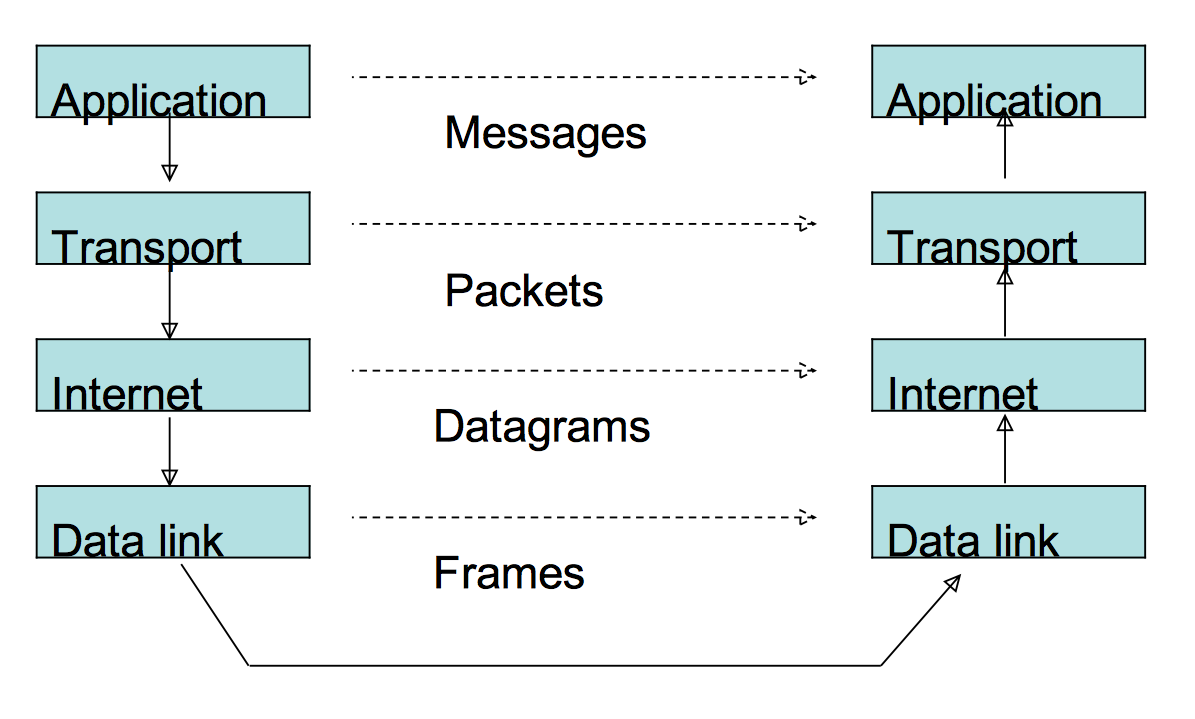
\includegraphics[width=100mm]{layering.png}
    		\caption{The TCP/IP Layered Structure}
    		\end{center}
    	\end{figure}
    	
    	\subsection{Ethernet}
    	Ethernet is a broadcast medium which has become the standard for local area networks. Ethernet stations communicate by sending each other data packets (individual blocks of data). Each Ethernet station is given a 48-bit MAC address to identify it on the network. With ethernet, every frame sent is received by every system connected to the Ethernet (including the transmitter).\\
    	
\noindent\textbf{Frame format:}
preamble - alternating 0s and 1s for synchronisation (8 octets), destination (6 octets), source (6 octets), frame type (2 octets), data (64-1500 octets), CRC (4 octets)
    	    	
\ \\ \textbf{Carrier Sense Multiple Access with Collision Detection (CSMA/CD):} Used to regulate access: A node waiting to transmits monitors the carrier signal waiting for the line to become idle, at which point it starts transmitting. If another node starts transmitting at the same time, the frame is garbled (detectable by the senders). When a collision is detected, each transmitting node ‘backs off’ for a random period. This randomness reduces chance of another collision (in the case of further collisions, the maximum period for back-off is doubled - exponential). As the network load increases, collisions become more frequent, causing more nodes to back off. This causes the network to slow down, but should not fail completely.
    	
    	\subsection{Internet Addresses}
    	Addresses are IPv4 (or 32-bit), consisting of 4 octets expressed as n.n.n.n (e.g. 127.0.0.1). The next-gen IPv6 (128-bit) consists of 6 octets (giving $\sim$1038 unique addresses).

• Address divided into network and machine number:
– subnet mask specifies how it is divided
    	
    	\subsection{ICMP}
	Internet Control Message Protocol (ICMP) is one of the core protocols of the Internet Protocol Suite. It is chiefly used by the operating systems of networked computers to send error messages indicating, for example, that a requested service is not available or that a host or router could not be reached. ICMP can also be used to relay query messages. It is assigned protocol number 1. ICMP differs from transport protocols such as TCP and UDP in that it is not typically used to exchange data between systems, nor is it regularly employed by end-user network applications (with the exception of some diagnostic tools like ping and traceroute).
	ICMP for Internet Protocol version 4 (IPv4) is also known as ICMPv4. IPv6 has a similar protocol, ICMPv6.

    	\subsection{RARP}
	Reverse Address Resolution Protocol is an obsolete computer networking protocol used by a host computer to request its       	Internet Protocol (IPv4) address from an administrative host, when it has available its Link Layer or hardware address, such as a MAC address.
	 It has been rendered obsolete by the Bootstrap Protocol (BOOTP) and the modern Dynamic Host Configuration Protocol (DHCP), which both support a much greater feature set than RARP.

    	\subsection{BOOTP}

	The Bootstrap Protocol, or BOOTP, is a network protocol used by a network client to obtain an IP address from a configuration server. The BOOTP protocol was originally defined in RFC 951.
	BOOTP is usually used during the bootstrap process when a computer is starting up. A BOOTP configuration server assigns an IP address to each client from a pool of addresses. BOOTP uses the User Datagram Protocol (UDP) as a transport on IPv4 networks only.	

	Historically, BOOTP has also been used for Unix-like diskless workstations to obtain the network location of their boot image in addition to an IP address, and also by enterprises to roll out a pre-configured client (e.g., Windows) installation to newly installed PCs.

	 Originally requiring the use of a boot floppy disk to establish the initial network connection, manufacturers of network cards later embedded the protocol in the BIOS of the interface cards as well as system boards with on-board network adapters, thus allowing direct network booting.

	 In 2005, users with an interest in diskless stand-alone media center PCs have shown new interest in this method of booting a Windows operating system.

 	The Dynamic Host Configuration Protocol (DHCP) is a more advanced protocol for the same purpose and has superseded the use of BOOTP. Most DHCP servers also function as BOOTP servers.
    	

	\subsection{DHCP}
	Dynamic Host Configuration Protocol  is a network configuration protocol for hosts on Internet Protocol (IP) networks. Computers that are connected to IP networks must be configured before they can communicate with other hosts. The most essential information needed is an IP address, and a default route and routing prefix. DHCP eliminates the manual task by a network administrator. It also provides a central database of devices that are connected to the network and eliminates duplicate resource assignments.

	  In addition to IP addresses, DHCP also provides other configuration information, particularly the IP addresses of local Domain Name Server (DNS), network boot servers, or other service hosts.

	 DHCP is used for IPv4 as well as IPv6. While both versions serve much the same purpose, the details of the protocol for IPv4 and IPv6 are sufficiently different that they may be considered separate protocols.[1]

	 Hosts that do not use DHCP for address configuration may still use it to obtain other configuration information. Alternatively, IPv6 hosts may use stateless address autoconfiguration. IPv4 hosts may use link-local addressing to achieve limited local connectivity.


    	\subsection{Transport layer}
	 In computer networking, the transport layer or layer 4 provides end-to-end communication services for applications[1] within a layered architecture of network components and protocols. The transport layer provides convenient services such as connection-oriented data stream support, reliability, flow control, and multiplexing.
	
	 The most well-known transport protocol is the Transmission Control Protocol (TCP). It lent its name to the title of the entire Internet Protocol Suite, TCP/IP. It is used for connection-oriented transmissions, whereas the connectionless User Datagram Protocol (UDP) is used for simpler messaging transmissions. TCP is the more complex protocol, due to its stateful design incorporating reliable transmission and data stream services. Other prominent protocols in this group are the Datagram Congestion Control Protocol (DCCP) and the Stream Control Transmission Protocol (SCTP).


    	\subsection{Name resolution/DNS}
	Domain Name System  is a hierarchical distributed naming system for computers, services, or any resource connected to the Internet or a private network. It associates various information with domain names assigned to each of the participating entities.

	  A Domain Name Service resolves queries for domain names (which are easier to understand and utilize when accessing the internet) into IP addresses for the purpose of locating computer services and devices worldwide.

	 An often-used analogy to explain the Domain Name System is that it serves as the phone book for the Internet by translating human-friendly computer hostnames into IP addresses. For example, the domain name www.example.com translates to the addresses 192.0.43.10 (IPv4) and 2620:0:2d0:200::10 (IPv6).
	
	The Domain Name System distributes the responsibility of assigning domain names and mapping those names to IP addresses by designating authoritative name servers for each domain. Authoritative name servers are assigned to be responsible for their particular domains, and in turn can assign other authoritative name servers for their sub-domains. This mechanism has made the DNS distributed and fault tolerant and has helped avoid the need for a single central register to be continually consulted and updated.

	 In general, the Domain Name System also stores other types of information, such as the list of mail servers that accept email for a given Internet domain. By providing a worldwide, distributed keyword-based redirection service, the Domain Name System is an essential component of the functionality of the Internet.

	 Other identifiers such as RFID tags, UPCs, international characters in email addresses and host names, and a variety of other identifiers could all potentially use DNS.

	 The Domain Name System also specifies the technical functionality of this database service. It defines the DNS protocol, a detailed specification of the data structures and communication exchanges used in DNS, as part of the Internet Protocol Suite.

  	\section{How is it implemented}
  	
    	\subsection{Java}
    	
      		\subsubsection{Client/server}
      		Many concurrent systems are implemented as client/server systems, where a server provides a service, and clients communicate with the server to use the service (e.g. web servers and web browsers, time servers providing synchronised time). Java comes with the \emph{java.net} package which contains many network-related classes.
      		
      		\subsubsection{TCP/IP}
      		The Transmission Control Protocol over Internet Protocol allows you to connect to a specific `port' on a remote machine, and read/write data to the port (like writing to a file). TCP is similar to a phone conversation: you connect, communicate and disconnect.     		
        	\subsubsection{Sockets}
        	A socket connects to a server, and Input/OutputStreams are used to read and write the data.
        	
        	\subsubsection{Socket servers}
        	Socket servers bind to a particular port and wait for someone to connect, at which point it communicates with the client. Server sockets can be set to timeout (\emph{setSoTimeout(5000);}) so that they don't wait indefinitely for a connection.
        	
      		\subsubsection{UDP (Sockets, Packets)}
      		The User Datagram Protocol doesn't carry the same guarantee for communication: a message isn't guaranteed to reach its destination. Data is sent as an individual `packet', rather than a continuous stream of data. Having sent a request, a response may be sent (or not). As there isn't necessarily a response, the socket should be set to timeout. UDP is more efficient than TCP, and allows for data to be `multicasted' to multiple recipients. Multicasting allows broadcasting to recipients whose individual addresses aren't necessarily known. UDP is particularly relevant in video streaming for example, where it doesn't matter if odd packets (or frames) are lost.
    	
\chapter{Real-time}
  	\section{What is a real-time system}
  	
  	All computer systems model some aspect of the outside world, although the timescale doesn't necessarily match that of the real world. Real time systems are required to conform to timescales imposed by the outside world: they must work as `fast' (or `slowly') as the outside world.
  	
  	\paragraph{Hard real time}: very tight deadlines; failure to meet deadlines is catastrophic (e.g. aerospace autopilot).
  	
  	\paragraph{Soft real time}: deadlines are more flexible; failure to meet deadlines is not necessarily catastrophic (e.g. multimedia video display applications, financial payroll systems).
  
  	
  	\section{Embedded systems}
  	Real time systems are often computer systems which are part of (embedded in) a larger system (e.g. process control, autopilot, manufacturing). ‘Embedded’ often used as a synonym for real time.
  	
  	\section{Characteristics}
  	
  	\begin{itemize}
  		\item Needs to cope with a variety of external events (where software is becoming frequently large and complex)
		\item Reliable and safe: able to detect and recover from failures
		\item Need to interact with external hardware
  		\item Need to be able to specify timing requirements (when to perform actions, when to complete actions by, what to do when deadlines are missed, importance of granularity (e.g. IBM PC clock granularity is 55ms, which can mean 100yds at 600mph)
  		\item Event-driven rather than process-driven (external events must be dealt with as they occur; event ordering is not generally predictable)
		\item Generally uses concurrent processes (each event source can be handled by a separate process)  
  		\item Must have predictable response times (factors to consider: caching/pipelining affect program speed, worst case is an order of magnitude slower than the average, fast programs \& external time)
  		\item Code must be safe (i.e. nothing `bad' will happen) and live (i.e. something `good' will eventually happen). `Eventually' must be able to be upper-bounded, as livelock can particularly be an issue in real-time systems.
  	\end{itemize}
  	
\chapter{Security}

	Computers have become an indispensable part of modern life, and failures can have serious consequences. In addition to the obvious loss/corruption of information which can occur, system failures can also lead to financial loss and serious injury or even a loss of life (in the case of failure of an aircraft's autopilot for example).
	
	Security issues can arise for various reasons, from basic hardware failures, programmatic errors, or even as a result of attacks by malicious parties. To prevent these sorts of failures, the hardware should provide at least a basic level of security (for example memory protection). These mechanisms should be utilised effectively by the OS.
	
	\section{Password Protection} 
	
	One of the most basic forms of security, passwords are used to verify users, and grant access to restricted resources. Only the individual user should have knowledge of the password (system admins should be able to change it if necessary, but not access it). Obviously the sysadmin's password is most important of all, as it allows unrestricted access to the system. It also requires special security measures, as a loss of the password could cause admins to be locked out of the system. Measures include storing a copy of the password in a safe location, or breaking the password into chunks, and distributing it so that no one person can reconstruct it. 
	
	For security reasons, a system should not show a password when typed in by the user (even displaying passwords as a series of asterisks reveals their length). Additionally, passwords should be encrypted by the system. A one-way encryption method could be used, as the entered password would only need to be compared to a stored copy of the encrypted password. An example of a one-way encryption algorithm is the \emph{Message Digest Version 5} (MD5). With MD5, the text is converted into a 16 byte value (a hash which is unique representation of the password in the majority of cases - the SHA256 checksum provides even greater reliability).
	
	\emph{Other forms of authentication include physical authentication (swipe cards, keys etc.), biometric data (fingerprints, iris patterns, face recognition etc.), and individual biometric actions (such as the timing of keystrokes when typing a password to recognise a user's behaviour)}

	\section{Encryption}
    	\subsection{Public-key}
    	\subsection{Steganography}
    	\subsection{SSL}
  	\section{Types of attack}
	    	\subsection{Trojan}
 		 A useful program which performs some extra unwanted activity e.g. copying your password file to a third party Many Trojans used for password cracking e.g. a Trojan might mimic a login dialog and send the password entered to a third party it might replace the system login program with a ‘doctored’ copy. Windows uses Ctrl-Alt-Del to prevent this.

    		\subsection{Virus}
Viruses embed themselves in other programs they might attach themselves to the end of an executable file and modify the program start address to run the virus code first. When they run, they copy themselves to other programs Only executable programs can be infected but: e.g. Word documents can contain executable macros.

	    	\subsection{Worm}
			Worms copy themselves from one machine to another usually exploiting loopholes in network code 
			\subsubsection{The Internet worm} released by Robert Morris Jr. of Cornell University brought the whole Internet to a halt for three days in 1998. The worm transferred a small ‘grappling hook’ program to neighboring machines.
The grappling hook then downloaded the rest of the worm which included a password cracker this then used Cracked passwords to connect to other machines, repeating the process. 


	    	\subsection{Denial of service}
			A website is flooded with requests which prevent legitimate request from being serviced

			can be a distributed denial of service, where machines around the work are hijacked by a Trojan to mount a coordinated attack. Due to the natured of this attack it is very hard to assess which requests are coming from a valid source as some botnets can have millions of emails. This type of attack is very commonly used by hacktavist groups such as anonymous and lulsec.

	    	\subsection{Mail bombing}

			Mail bombing is similar to a Denial of service attack however in this instance a users email address is rendered unaccessible.

Mail bombing can be performed in a variety of ways one such is \textbf{Mass Mailing} this entails sending a vast amount of emails to a users account causing an overflow in the users inbox or exceeding the maximum amount of storage on the server which would stop legitimate emails from reaching there intended location.

\textbf{List Linking} is the process of signing a user up to several email lists which the victim will then have to unsubscribe from, this type of mail bombing can be circumnavigated by making the user confirm their subscription to the mailing list, however if the attacker uses a forwarding email account this method is ineffective. 

\textbf{Zip bombing} is performed by sending a zip archive that may only consist of one letter repeated an extremely large amount of times, such a file will be extremely small when archived however the anti virus on the server will attempt to open the archive will result in a massive amount of processing time being required by the server resulting in a denial of service attack. 


	    	\subsection{Phishing}
		Spam directing users to fake websites (usually copied from real ones) e.g. bank sites: used to collect account details form submission transfers you to the real site (after your account details have been recorded by the bad guys).


	    	\subsection{Keylogging}
  		 A Trojans records your keystrokes (password etc.) and transmits them to a remote site.

		\subsection{DNS poisoning and pharming}
		DNS entries are changed so a legitimate domain name gets redirected to a fake site.

		\subsection{Man in the middle attacks}
Man in the middle attack is a form of active eavesdropping in which the attacker makes independent connections with the victims and relays messages between them, making them believe that they are talking directly to each other over a private connection, when in fact the entire conversation is controlled by the attacker. The attacker must be able to intercept all messages going between the two victims and inject new ones, which is straightforward in many circumstances (for example, an attacker within reception range of an unencrypted Wi-Fi wireless access point, can insert himself as a man-in-the-middle

A man-in-the-middle attack can succeed only when the attacker can impersonate each endpoint to the satisfaction of the other—it is an attack on (or lack of) mutual authentication. Most cryptographic protocols include some form of endpoint authentication specifically to prevent MITM attacks. For example, SSL can authenticate one or both parties using a mutually trusted certification authority.

		\subsection{General intrusions}
		Using a compromised server to store illicit material (e.g. porn or pirated movies)


	  	\section{Protection}
		
		\subsection{Java Security}
		Java applets are loaded into a JVM using a security manager which: statically scans bytecodes looking for unsafe code, e.g. jumps to addresses in a different method, dynamically checks resource requests, and grants or denies them.

		``Trusted" code can be digitally signed, signatures are verified by the security manager.

		Stack inspection used to propagate permissions callers must be trusted and must have the required permission.


 		\subsection{Sandboxes}
		 e.g. an emulator, or a virtual machine like the JVM any damage affects only the sandbox, not the host machine.
		The sandbox typically provides a tightly-controlled set of resources for guest programs to run in, such as scratch space on disk and memory. Network access, the ability to inspect the host system or read from input devices are usually disallowed or heavily restricted. In this sense, sandboxes are a specific example of virtualization.

		\subsection{Firewalls}
		Prevent network attacks by using a firewall to filter network traffic, e.g. by restricting access to certain ports only machines inside the firewall can still communicate freely.
		Firewalls can also do packet filtering e.g. inspect packet contents for virus checking or spam blocking purposes

		\subsection{Proxies}
		Send all outbound traffic via a proxy. The proxy passes on requests to the outside world and routes replies back to the originator.
		Only the proxy is visible to the outside world.
		Other machines are prevented by a firewall from contacting the outside world directly.


\end{document}
